\documentclass[xcolor=dvipsnames]{beamer}  

\input{slides_preamb.tex}

\title{Computational Economics Assignment}

\author{John Stachurski}

\date{April 2026}


\subtitle{Ergodicity}


\begin{document}

\begin{frame}
  \titlepage
\end{frame}

\begin{frame}
    
    This document begins with a short introduction to ergodic chaos

    \vspace{0.5em}
    \vspace{0.5em}
    \vspace{0.5em}
    Assignment exercises are at the end

\end{frame}


\begin{frame}
    
    Consider the one-dimensional dynamic system
    %
    \begin{equation}\label{eq:quad_map}
        x_{t+1} = g(x_t) 
        \quad \text{ where } \quad g(x) := 4x(1-x).
    \end{equation}
    %

    The law of motion in~\eqref{eq:quad_map} provides an update rule for the state
    $x_t$ and a \navy{trajectory} $(x_t)_{t\geq 0}$ recursively defined by
    $x_{t+1} = g(x_t)$ and some fixed initial condition $x_0$

    \vspace{0.5em}
    Another way to write this trajectory is
    %
    \begin{equation*}
        x_t = g^t (x_0) 
        \quad \text{where} \quad
        g^t := g \circ \cdots \circ g
    \end{equation*}
    %

    The product on the right is $t$ compositions of $g$ with itself.

    \vspace{0.5em}
    The map $g$ is called either the \navy{logistic map} or the \navy{quadratic
    map} 

\end{frame}


\begin{frame}

    \begin{figure}
        \centering
        \scalebox{0.5}{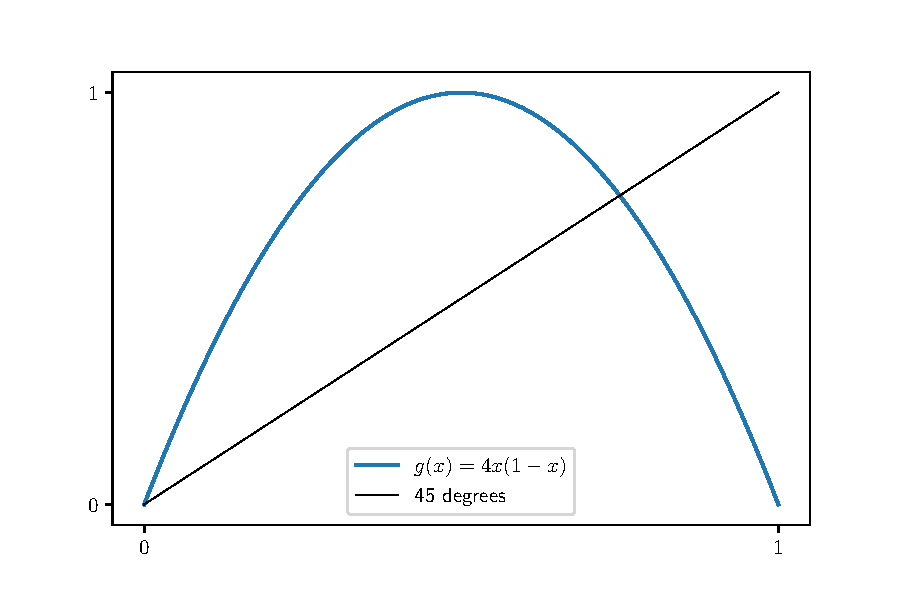
\includegraphics{figures/chaos_intro_quad_map.pdf}}
        \caption{\label{f:chaos_intro_quad_map} The quadratic map and 45 degree line}
    \end{figure}

\end{frame}


\begin{frame}
    
    The 45 degree diagram on the previous slide suggests that cycles occur when
    we iterate with the quadratic map 

    \vspace{0.5em}
    This is easily confirmed by plotting time series

    \vspace{0.5em}
    The next figure shows one such series when $x_0 = 0.3$

    \vspace{0.5em}
    We see that the behavior of the state is not only cyclical but also highly erratic

    \vspace{0.5em}
    It shows no sign of convergence to regular behaviour   

\end{frame}


\begin{frame}
    
    \begin{figure}
        \centering
        \scalebox{0.5}{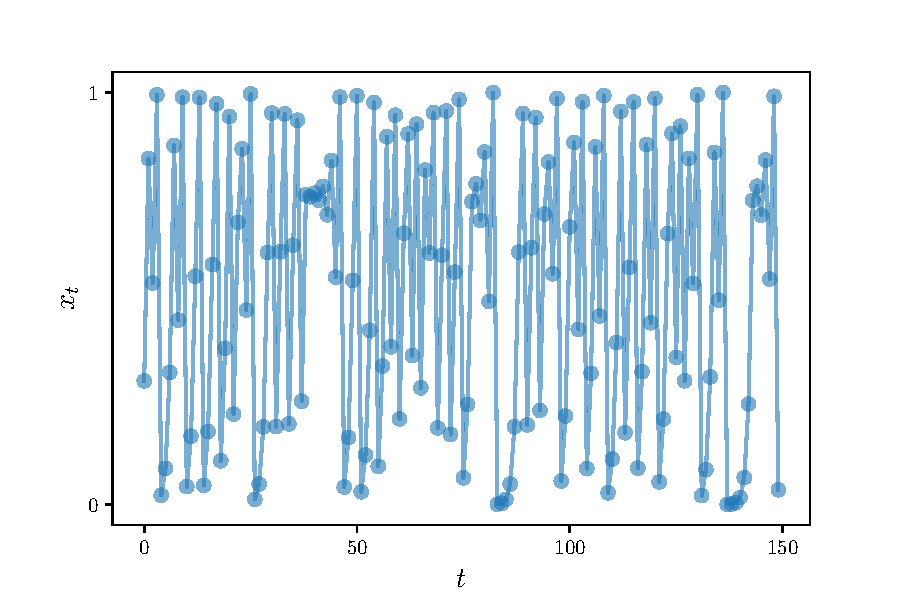
\includegraphics{figures/chaos_intro_traj.pdf}}
        \caption{\label{f:chaos_intro_traj} Time series from the quadratic map when $x_0 = 0.3$}
    \end{figure}


\end{frame}


\begin{frame}
    

    The figure on the next slide shows $x_t = g^t(x_0)$ as a function of the
    initial condition $x_0$

    Specifically, we set

    \begin{itemize}
        \item $x_0$ ranges across a grid of 100 points in $(0,1)$
        \item $n=20$
    \end{itemize}

    Thus, the figure shows how the forecast state 20 periods hence changes with
    the initial condition

    Evidently there is great variability

    Thus, we have sensitive dependence on initial conditions

    If this is a model for some aggregate quantity, then we can say almost
    nothing in terms of useful predictions, since the initial condition will
    almost always be measured with some degree of error


\end{frame}


\begin{frame}
    
    \begin{figure}
        \centering
        \scalebox{0.5}{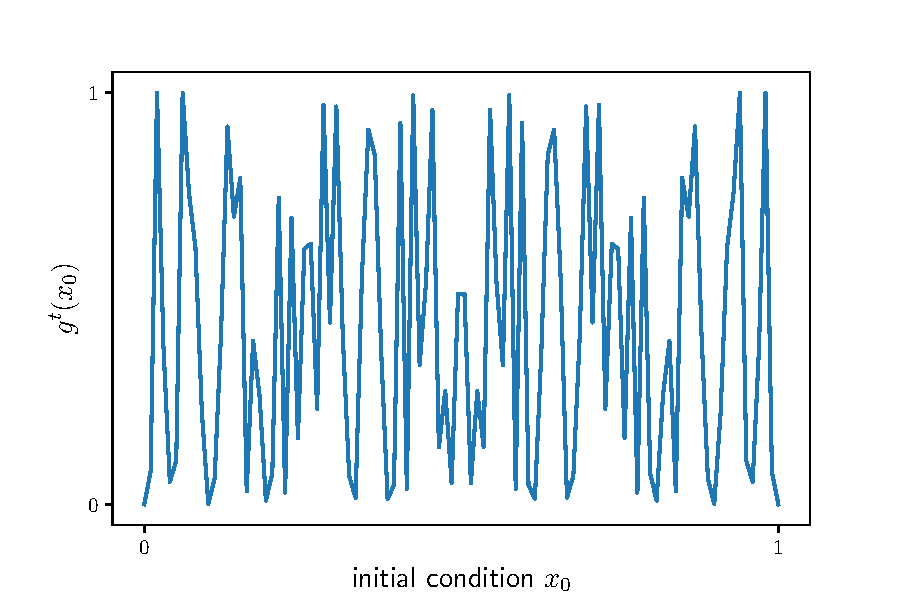
\includegraphics{figures/chaos_intro_quad_map_iter.pdf}}
        \caption{\label{f:chaos_intro_quad_map_iter} The time $t$ state as a
        function of the initial condition}
    \end{figure}

\end{frame}



\begin{frame}
    
    At the same time, the model can generate strong ``statistical'' predictions 
    over long time horizons

    As one way to see this, consider the histogram shown in the next figure

    This is a histogram of the sequence $(g^t(x_0))_{t=0}^n$ when $x_0=0.3$ and
    $n=100,000$

    Evidently there is some pattern to the apparent randomness, since the
    histogram is symmetric and U-shaped

    Moreover, if we choose an alternative initial condition and reproduce the
    histogram, then, apart from a few special cases (e.g., $x_0 = 0$), exactly
    the same pattern arises

    Hence, at the level of distributions, sensitive dependence on initial conditions disappears

\end{frame}



\begin{frame}
    
    \begin{figure}
        \centering
        \scalebox{0.5}{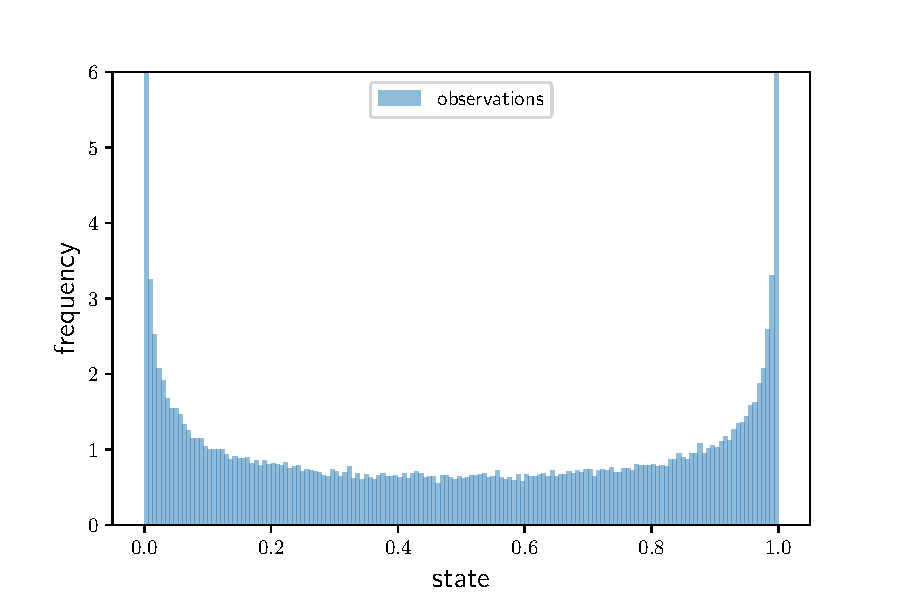
\includegraphics{figures/chaos_intro_time_series_hist.pdf}}
        \caption{\label{f:chaos_intro_time_series_hist} A histogram of $(x_0,
        \ldots, x_n)$ when $n=100,000$}
    \end{figure}

\end{frame}



\begin{frame}
    
    The shape of the histogram becomes clearer as the length of the time series increases

    In fact, there is a specific limit to this process: the histograms are
    converging on $(0, 1)$ to the function
    %
    \begin{equation}\label{eq:fstarpf}
        \psi^*(x) := \frac{1}{\pi \sqrt{x (1-x)}}
        \qquad (x \in (0,1))
    \end{equation}
    %

    The function $\psi^*$ is called the \navy{arcsine distribution}

    The figure on the next slide illustrates converges of the histogram
    to $\psi^*$ as $n \to \infty$ by jointly plotting the histogram of an even
    longer time series and the density $\psi^*$


\end{frame}

\begin{frame}
    
    \begin{figure}
        \centering
        \scalebox{0.5}{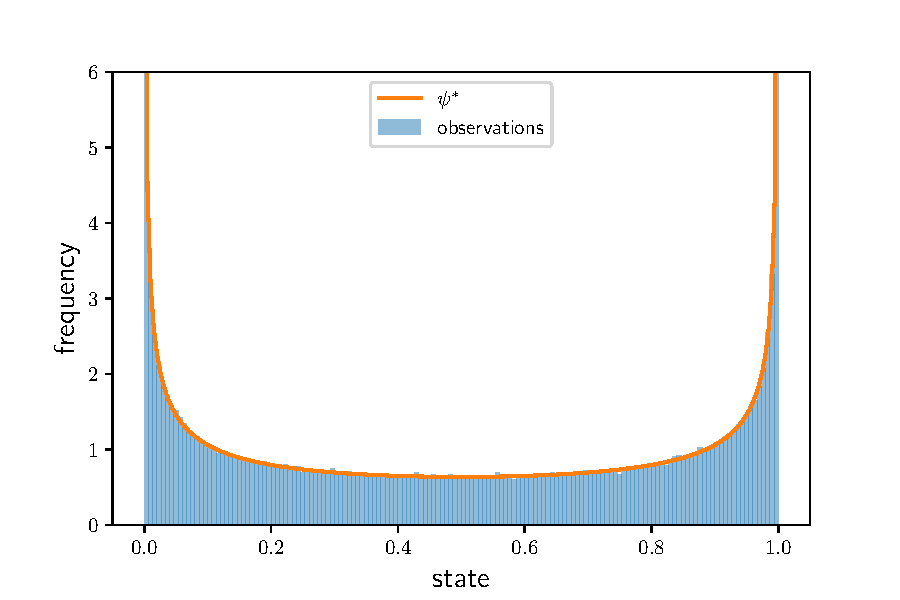
\includegraphics{figures/chaos_intro_time_series_hist_fstar.pdf}}
        \caption{\label{f:chaos_intro_time_series_hist_fstar} Histogram of a
        length $250,000$ trajectory and the stationary density $\psi^*$}
    \end{figure}


\end{frame}



\begin{frame}

    In fact one can also show that, for any
    bounded function $h$  we have
    %
    \begin{equation}\label{eq:berg}
        \frac{1}{m} \sum_{t=1}^m h(g^t(x_0))
        \to 
        \int h(x) \psi^*(x) \diff x 
        \qquad (m \to \infty)
    \end{equation}
    %
    for $\psi^*$-almost-every $x_0$

    \medskip
    \medskip
    
    The result in \eqref{eq:berg} is a version of the celebrated \navy{Birkhoff ergodic
    theorem}, proved by George David Birkhoff (1884--1944) in 1931, 
    which verified fundamental claims in the field of statistical mechanics.

\end{frame}




\begin{frame}
    \frametitle{Cross-sectional data}
    
    \vspace{0.5em}
    Suppose $x_t^i$ is a measurement related to individual $i$ in a cohort of $n$
    agents

    \vspace{0.5em}
    For simplicity, let's call it ``wealth''

    \vspace{0.5em}
    Suppose each individual's wealth updates as $x_{t+1}^i = g(x_t^i)$

    \vspace{0.5em}
    We take as given the initial states $(x_0^i)_{i=1}^n$, representing
    the cross-sectional wealth distribution at time zero

    \vspace{0.5em}
    Then we forecast the time $t$ wealth distribution
    by computing $(g^t(x_0^i))_{i=1}^n$


\end{frame}


\begin{frame}
    

    The next figure shows three forecasts corresponding to three
    different initial distributions. 

    \vspace{0.5em}
    Each row, containing a left and right subfigure, was constructed as follows

    \begin{itemize}
        \item an initial density $\psi_0$ was chosen
        \item $100,000$ observations $(x_0^i)_{i=1}^n$ were drawn from $\psi_0$
        \item the cross section was shifted forward to time $t=50$ by computing
        $(g^t(x_0^i))_{i=1}^n$
    \end{itemize}

   On the left, we show the density $\psi_0$ that was used to generate the draws
   and the histogram of draws

   On the right we show the histogram of $(g^t(x_0^i))_{i=1}^n$ and $\psi^*$ 


    The three initial densities are Beta$(2,2)$, Beta$(2,5)$, and Beta$(5,2)$

\end{frame}

\begin{frame}
    
    \begin{figure}
        \centering
        \scalebox{0.30}{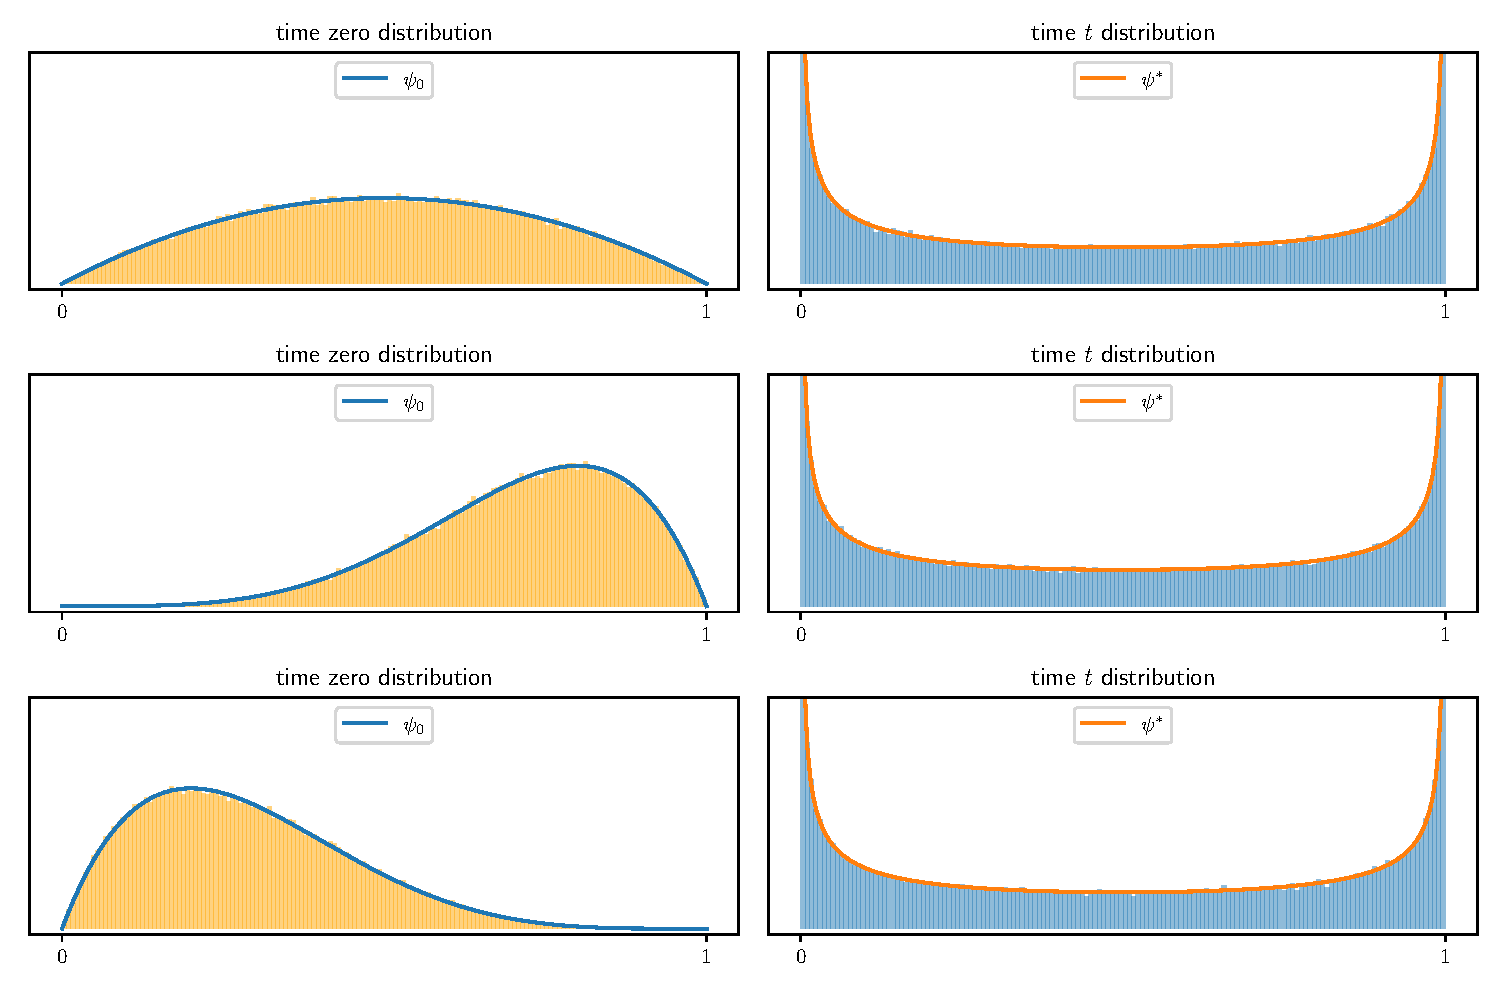
\includegraphics{figures/chaos_intro_hists.pdf}}
        \caption{\label{f:chaos_intro_hists} Initial (left) and predicted
        (right) cross-sectional distributions}
    \end{figure}


\end{frame}

\begin{frame}
    
    The initial distributions are represented as histograms on the left hand side
    of the figure

    \medskip
    It is apparent from the figure that (a) the
    forecast distributions display significantly more regularity that the initial
    conditions, and (b) the forecast cross-sectional distributions look very
    similar to the distribution generated from a single time series

    \medskip
    More specifically, the simulations show that the cross-sectional histograms
    also converge to $\psi^*$ as the number of countries and forecast date
    become large


    \medskip
    This connection between cross-sectional averages and time series averages is
    called \emph{ergodicity}.

\end{frame}

\begin{frame}
    
    {\bf Exercise 1} Produce a Jupyter notebook where you replicate all figures
    in the graph

    \medskip
    Do this
    %
    \begin{enumerate}
        \item Using Numba for the computations
        \item Using JAX for the computations
    \end{enumerate}

    Pay attention to the quality of your code!

    \medskip
    \begin{itemize}
        \item See \url{https://python-programming.quantecon.org/writing_good_code.html}
        \item Use good Numba/JAX style
    \end{itemize}


    Use markdown cells to add commentary -- explain what the figures are.

\end{frame}


\begin{frame}
    
    {\bf Exercise 2} Adding to the same Jupyter notebook, shift a cross-section $(x_0^i)_{i=1}^n$
    forward in time $t$ periods

    \begin{enumerate}
        \item draw $(x_0^i)_{i=1}^n$ as IID samples from Uniform$(0,1)$
        \item compute the updated cross section $(g^t(x_0^i))_{i=1}^n$
    \end{enumerate}

    Perform step 2 as quickly as possible 
    %
    \begin{enumerate}
        \item using Numba for the computations
        \item using JAX for the computations --- use a GPU on Colab
    \end{enumerate}

    Time your solution with the following settings

    \begin{itemize}
        \item $n = 10,000,000$
        \item $t = 100$
    \end{itemize}

    Use 64-bit float throughout, aim for speed and clarity

\end{frame}


\end{document}









